\documentclass[12pt]{article}


% defining image path
\usepackage{graphicx}
\graphicspath{ {./images/} }

% tables
\usepackage[utf8]{inputenc}
\usepackage[table]{xcolor}
\usepackage{enumitem}
\usepackage{multirow}
% \usepackage{multicol}
% \usepackage{adjustbox}
% \usepackage{tabularx}
% \newcolumntype{L}{>{\raggedright\arraybackslash}X}
\setlist{nolistsep}

% rotate page
\usepackage{pdflscape}

\pagestyle{empty}
\setcounter{secnumdepth}{2}


\topmargin=0cm
\oddsidemargin=0cm
\textheight=22.0cm
\textwidth=16cm 

\parindent=0cm
\parskip=0.15cm
\topskip=0truecm
\raggedbottom
\abovedisplayskip=3mm
\belowdisplayskip=3mm
\abovedisplayshortskip=0mm
\belowdisplayshortskip=2mm
\normalbaselineskip=12pt
\normalbaselines

\begin{document}
\vspace*{0.5in}
\centerline{\bf\Large
Requirements for the Kakuro project}


\vspace*{0.5in}
\centerline{\bf\Large Iteration 2 COMP354}

\vspace*{0.5in}
\centerline{\bf\Large Team PK-A}

\vspace*{0.5in}
\centerline{\bf\Large 15 March 2020}

\vspace*{1.5in}
\begin{table}[htbp]
\caption{Team Members}
\begin{center}
\begin{tabular}{|c |c | c|}
\hline
Name & Role & ID Number \\
\hline\hline
Tiffany Ah King & Quality Control & 40082976 \\
\hline
Isabelle Charette & Documenter & 40008121 \\
\hline
Brian Gamboc-Javiniar & Coder & 40033124 \\
\hline
Vsevolod Ivanov & Organizer & 40004286 \\
\hline
Chang Liu & Quality Control & 40056360 \\
\hline
Nolan Mckay & Coder & 27873557 \\
\hline
Nalveer Moocheet & Quality Control & 40072605 \\
\hline
Hoang Thuan Pham & Coder & 40022992 \\
\hline
Audrey-Laure St-Louis & Documenter & 27558783 \\
\hline
Jia Ming Wei & Documenter & 40078192 \\
\hline
\end{tabular}
\end{center}
\end{table}


\newpage

\renewcommand*\contentsname{Table of Contents}

\tableofcontents

\clearpage

\section{Introduction}

\subsubsection{Purpose}
The purpose of this document is to present the design of the Kakuro game for the course COMP 354. 

\subsubsection{Scope}
This document is intended to provide detailed design specifications of the Kakuro game.

\newpage

\section{Architectural Design} \label{sec:arch}




\begin{figure}[htbp]
    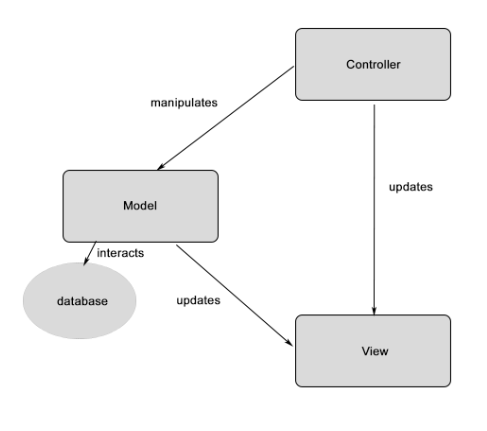
\includegraphics[width=0.7\textwidth]{archi_diagram}
    \caption{Architecture Diagram}
    \label{fig:archi_diagram}
\end{figure}

\subsection{Rationale}

The architecture chosen for the Kakuro game is the Model View Controller model (MVC). The MVC architecture is constructed of three separate components: the model, the view and the controller. \newline

The model is the central component of the game. It stores the data and it changes depending on the state of the game. In Kakuro, the model stores the information of the cells from the rows and the columns displayed by the graphical user interface. The view is the graphical user interface (GUI) of the game. It displays the grid, the buttons, and the text elements but it also displays the date from the model. It allows the player to enter numbers to play the game. Whenever the model changes, the GUI reacts to these changes by updating itself. For example, if the player presses the button restart, the model will be updated by clearing its input cells and therefore, the GUI will react by showing empty input cells to the user.\newline

The controller manages the interactions with the user and decides which functions should be called given an action. The controller will use the model’s data, he will take action on those depending on the user’s action and he will send it to the view for it to show it in the GUI.\newline


\subsection{Subsystem Interface Specifications}

\subsubsection{2.2.1 View Interface}

2.2.1.1 GameView \newline

The GameView class is the interface used for the View. With its constructor, it initializes the GUI of our Kakuro game. The following methods are available for this interface:
\newline
\begin{itemize}
\item getBoardUI (Cell)
\item getMaxNumberValid()
\item getMinNumberValid()
\item getNumberFormatterClassType()
\item getSavedInput()
\item hideBoard()
\item settingTextField(JTextField)
\item showBoard()
\item updateView()\newline
\end{itemize} 


2.2.1.2 MenuBarView\newline

The MenuBarView class is used for the different buttons displayed on the GUI of the game. The MenuBarView class contains the following methods:
\newline
\begin{itemize}
\item buttonsSetUp()
\item getMainPannel()
\item toggleMenu() \newline
\end{itemize}

2.2.1.3 ChronoView\newline

The ChronoView class handles the chronometer of the game. It contains the following methods:\newline
\begin{itemize}
\item getTimerLabel()
\item setTimerLabel()\newline
\end{itemize}


\subsubsection{2.2.2 Model Interface}
The interface between the controller and model is called whenever the controller receives input from the player. The kakuro.models package contains all the classes from the model interface. The following methods are part of the interface:\newline

2.2.2.1 GameModel \newline

The GameModel class is the interface used for the Model of our system. It interacts with the database and it handles all the functions that are implementing the rules of the game. It contains the following methods:\newline
\begin{itemize}
\item getColumns(int, int)
\item getRows()
\item initBoard()\newline
\end{itemize}

2.2.2.2 ChronoModel\newline

The ChronoModel class is the model of the chronometer of our Kakuro game. It contains the following methods:\newline
\begin{itemize}
\item getDelay() : Returns the delay used for the chronometer
\item getHours() : Returns the hours value of the chronometer
\item getMinutes(): Returns the minutes value of the chronometer
\item getSeconds() Returns the seconds value of the chronometer
\item resetTimer() : Brings the chronometer to the value zero for its seconds, minutes and hours
\item setHours() : Sets the hours of the chronometer
\item setMinutes() : Sets the minutes of the chronometer
\item setSeconds() : Sets the seconds of the chronometer
\item updateTime()\newline
\end{itemize}

2.2.2.3 PlayerModel\newline

The PlayerModel class handles the player’s information. It contains the following methods:\newline
\begin{itemize}
\item getPlayerPassword() : Returns the password of the player
\item getPlayerUsername() : Returns the username of the player
\item setPlayerPassowrd() : Sets the password of the player
\item setPlayerUsername(): Sets the username of the player\newline
\end{itemize}





\subsubsection{2.2.3 Controller Interface}

The controller interface is a package (kakuro.controllers) composed of the following three classes:\newline

2.2.3.1 GameController\newline
The controller accepts input from the player and performs simple validations on it. The class contains the following methods : \newline
\begin{itemize}
\item connectDatabase() : Connects the game to the database
\item disconnectDatabase() : Disconnect the database from the game
\item getDatabaseConnection() : Returns the connections established from the database.
\item getMaxNumberValid() : Returns the maximum number aloud for the player to use during the game
\item getMinNumberValid() : Returns the minimum value aloud for the player to use during the game
\item getNumberFormatterClassType()
\item initGame() : 
\item loadGame()
\item loadInputInModel
\item loadPreconfigureGame(int)
\item loopGame()
\item pause() : Pause the game which stops the chronometer and blocks the player from entering data in the game
\item restart() : Clears the board and restart the chronometer
\item resume() : Starts the chronometer and allows the player to continue playing by entering value in the board game
\item saveGame() : Save the state of the game in the database
\item solveBoard() : Solves the board by calculating the sums of the rows and the columns and checks if it brings to a correct solution. 
\item submit() : Lets the user get feedback from the system to know if he got the right solution or not \newline
\end{itemize}


2.2.3.2 MenuBarController\newline
The MenuBarController Class accepts input from the player through the menu bar and performs actions depending on the button that is being pressed. The class contains the following methods:\newline
\begin{itemize}
\item getButtonMenuView()
\item getView()
\item isPaused()
\item load()
\item loadPreconfigureGame(GameDifficulty g)
\item pause()
\item resume()
\item save()
\item submit()\newline
\end{itemize}



2.2.3.3 ChronoController\newline
\begin{itemize}
\item chronoPause() : Pause the chronometer
\item chronoStart() : Starts the chronometer
\item getHours() : Returns the hours of the chronometer
\item getMinutes() : Returns the minutes of the chronometer
\item getSeconds() : Returns the seconds of the chronometer
\item getView():  Returns the label of the chronometer.
\item hide() : Hides the chronometer on the GUI of the game.
\item resetTimer() : Resets the chronometer to bring it to zero (hours, minutes and seconds)
show() : Display the chronometer in the GUI of the game
\item timerSetUp() : Set up the chronometer by attaching an action listener to it.
\item toggleTimerDisplay() : Sets the chronometer visible or hides it dependanding on the state he’s in\newline
\end{itemize}

\subsubsection{2.2.4 Other}

To support our MVC architecture, we created the following classes. \newline

Core Package \newline

2.2.4.1 Cell \newline
\begin{itemize}
\item getFirstValue()
\item getSecondValue()
\item getType()
\item setFirstValue(int) \newline
\end{itemize}

2.2.4.2 DatabaseConnection \newline
\begin{itemize}
\item connect()
\item createGameProgressTable()
\item createGameTable()
\item createPlayerTable()
\item  disconnect()
\item  getConnection()
\item  insertMainPlayer()
\item  insertPlayerData()
\item  insertPreconfiguredGames() \newline
\end{itemize}

2.2.4.3 GameDifficulty\newline
\begin{itemize}
\item gameDifficultyToInt(GameDifficulty) : Transform the level of difficulty chosen to a integer value and returns it \newline
\end{itemize}

2.2.4.4 GameDifficultyListItem\newline
\begin{itemize}
\item getDifficulty(): Returns the level of difficulty chosen by the player
toString(): Returns a description of the difficulty chosen \newline
\end{itemize}

2.2.4.5 LinePanel\newline
\begin{itemize}
\item paintComponent(Graphics): Draws the diagonal line in the black cells
\item settingTxt(JTextField): Sets the background and the foreground color of the game \newline
\end{itemize}

2.2.4.6 Tools\newline
\begin{itemize}
\item arrayToNodes(DefaultMutableTreeNode)
\item childrenToArray(TreeNode)
\item randomInt() : Generates a random integer value \newline
\end{itemize}


2.2.4.7 UniquePartitions\newline
\begin{itemize}
\item fillCombinations(DefaultMutableTreeNode)
\item getTreeRoot() \newline
\end{itemize}

GameProgresse DAO package\newline

2.2.4.8 GameProgressDao\newline
\begin{itemize}
\item load(Connection, String)
\item save(Connection, String, Cell) \newline
\end{itemize}

Game DAO package\newline

2.2.4.8 GameDao\newline

\begin{itemize}
\item loadAllPreconfiguredGames(Connection) \newline
\end{itemize}


Player DAO package\newline

2.2.4.9 PlayerDAO\newline

\begin{itemize}
\item Login (Connection, String, String)
\item Register(Connection, String, String) \newline
\end{itemize}



\newpage

\section{Detailed Design} \label{sec:detail}

The Karuro system consists of three subsystems: Game-Puzzle, Registration, and Ranking subsystems. The Game-Puzzle subsystem is implemented in the iteration 1 and iteration 2. During the iteration 1, this subsystem is implemented using the UI and the console. During the iteration 2, a SQLite server is integrated in the libraries so that the input data and solution data are possible to be stored in the database. Therefore, having a database server is essential to implement the Registration subsystem and Ranking subsystem in the iteration 3. 

\begin{figure}[htbp]
    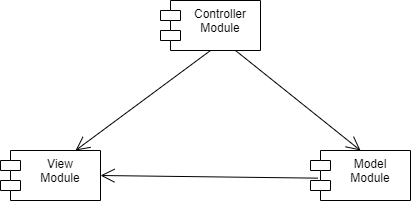
\includegraphics[width=1\textwidth]{Subsystems_UML}
    \caption{UML of Kakuro Subsystems}
    \label{fig:Subsystems_UML}
\end{figure}

The three subsystem are derived from the whole system, the Karuro system. On the other hand, the three subsystems are independent of each other. This design practice the principles of high cohesion and low coupling. The three subsystems are also three components of this software systems. The three subsystems present three different parts of view, apply different models, and use different parts of controller. The Ranking subsystem intersects with the Registration subsystem in the Player class, database connection class, and the MainFrame class, and both of them have dependency with the Game-Puzzle subsystem because the game scores come from the game puzzle.

\newpage

\begin{landscape}

\subsection{Game-Puzzle Subsystem}

\subsubsection{Detailed Design Diagram}

\begin{figure}[htbp]
    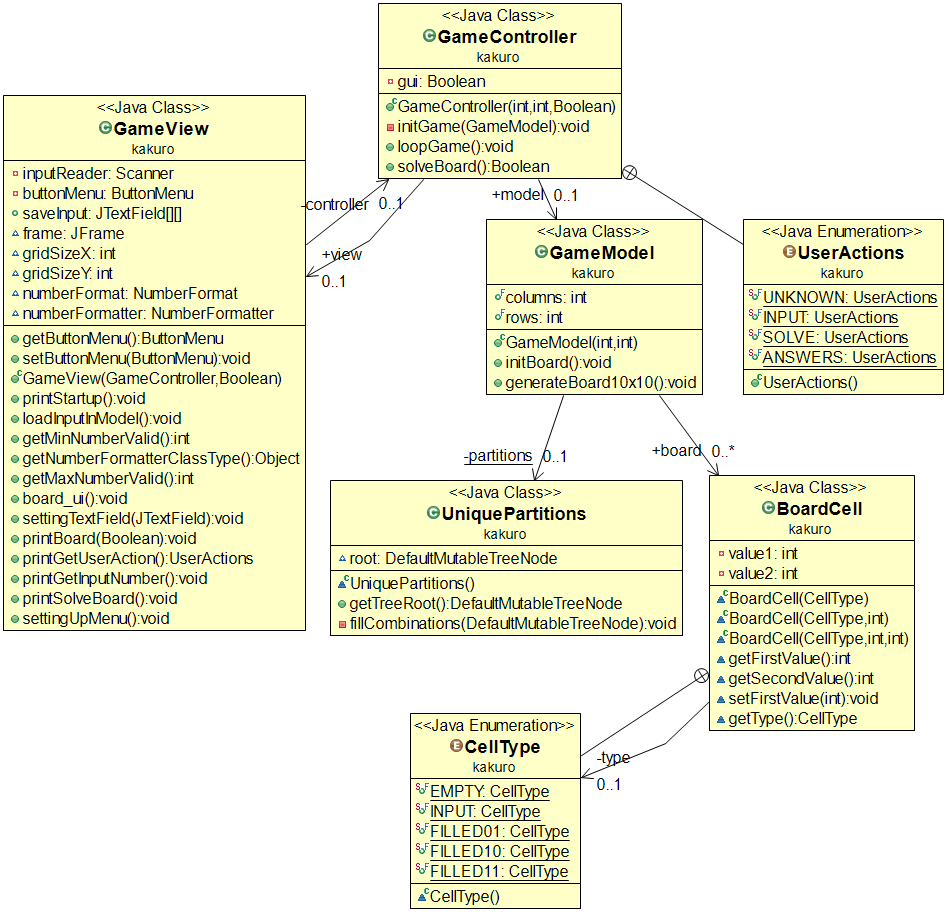
\includegraphics[width=1.5\textwidth, height=.7\textheight]{images/GamePuzzle_UML}
    \caption{UML of Geme-Puzzle Subsystems}
    \label{fig:GamePuzzle_UML}
\end{figure}

\end{landscape}

The Game-Puzzle subsystem design follows the MVC model. The GameView is the user interface of this system, it includes line\_panel, BoarCell, CellType and ButtonMenu classes. The Chrono class provides the timer function that is not used in this subsystem and will be used in the Ranking subsystem. The model part includes GameModel, UniquePartitions, Tools, and database part which includes GameDaoImpl and GameProgressDaoImpl. The Controller part is the GameController class. 

\subsubsection{Units Description}

\begin{flushleft}
\begin{tabular}{| l | l | l | l | l |}
    \hline
    \textbf{Class Name} & \multicolumn{4}{ l |} {\textbf{GameController}} \\
    \hline
    Inherits from & \multicolumn{4}{ l |}{None} \\
    \hline
    Description & \multicolumn{4}{ l |} {The controller of subsystem} \\
    \hline
    \multirow{4}{*}{Attributes} & Visibility & Data Type & Name & Description \\\cline{2-5}
     & Public & enum & UserActions & User actions \\\cline{2-5}
     & Public & DatabaseConnection & database & A database connection \\ \cline{2-5}
     & Private & Boolean & gui & GUI or console \\
    \hline
    \multirow{9}{*}{Methods} & Visibility & Method Name & \multicolumn{2}{l |}{Description} \\\cline{2-5}
    
    & Public & GameController(int, int, Boolean) & \multicolumn{2}{l |}{Constructor} \\
    \cline{2-5}
    & Public & loopGame() & \multicolumn{2}{l |}{A loop that keep game running} \\
    \cline{2-5}
    & Public & solveBoard() & \multicolumn{2}{l |}{To check if the answer is correct } \\
    \cline{2-5}
    & Private & initGame(GameModel) & \multicolumn{2}{l |}{To initiate a new game} \\ \cline{2-5}
    \cline{2-5}
    & Public & loadInputInModel(boolean) & \multicolumn{2}{l |}{Loads input to model} \\
    \cline{2-5}
    & Public & loadPreconfiguredGame(int) & \multicolumn{2}{l |}{Loads a configured game} \\ \cline{2-5}
    & Public & connectDatabase() & \multicolumn{2}{l |}{Connects to database} \\\cline{2-5}
    & Public & disconnectDatabase() & \multicolumn{2}{l |}{Disconnects to database} \\
    \hline
\end{tabular}
\end{flushleft}

\begin{flushleft}
\begin{tabular}{| l | l | l | l | l |}
    \hline
    \textbf{Class Name} & \multicolumn{4}{ l |} {\textbf{GameModel}} \\
    \hline
    Inherits from & \multicolumn{4}{ l |}{None} \\
    \hline
    Description & \multicolumn{4}{ l |} {The view of subsystem} \\
    \hline
    \multirow{3}{*}{Attributes} & Visibility & Data Type & Name & Description \\
    \cline{2-5}
    
     & Public & int & columns & The columns of the board \\
    \cline{2-5}
    & Public & int & rows & The rows of the board \\
    \hline
    \multirow{4}{*}{Methods} & Visibility & Method Name & \multicolumn{2}{l |}{Description} \\
    \cline{2-5}
    & Public & GameModel(int, int) & \multicolumn{2}{l |}{Constructor} \\
    \cline{2-5}
    & Public & initBoard() & \multicolumn{2}{l |}{To initiate a new board} \\
    \cline{2-5}
    & Public & generateBoard10x10() & \multicolumn{2}{l |}{To generate a 10x10 board} \\
    \hline
\end{tabular}
\end{flushleft}

\newpage
\begin{flushleft}
\begin{tabular}{| p{2cm} | l | l | l | p{58.8mm} |}

    \hline
    \textbf{Class Name} & \multicolumn{4}{ l |} {\textbf{GameView}} \\
    \hline
    Inherits from & \multicolumn{4}{ l |}{None} \\
    \hline
    Description & \multicolumn{4}{ l |} {The view of the subsystem} \\
    \hline
    \multirow{9}{*}{Attributes} & Visibility & Data Type & Name & Description \\
    \cline{2-5}
     & Private & Scanner & inputReader &  A input reader \\\cline{2-5}
     & Private & ButtonMenu & buttonMenu & A ButtonMenu object \\ \cline{2-5}
     & Private & JFrame & frame & A JFrame object \\ \cline{2-5}
     & Public & JTextField[][] & saveInput & The inputs array\\ \cline{2-5}
     & Private & int & gridSizeX & X value of grid size \\ \cline{2-5}
     & Private & int & gridSizeY & Y value of grid size \\ \cline{2-5}
     & Private & NumberFormat & numberFormat & A number format instance \\ \cline{2-5}
     & Private & NumberFormatter & numberFormatter & A NumberFormatter instance \\ 
    \hline
    \end{tabular}
    \begin{tabular}{| p{2cm} | l | l | l | p{5cm} |}
    \multirow{16}{*}{Methods} & Visibility & Method Name & \multicolumn{2}{l |}{Description} \\
    \cline{2-5}
    & Public & GameView(GameController, Boolean) &  \multicolumn{2}{l |}{Constructor} \\\cline{2-5}
    & Public & getButtonMenu() & \multicolumn{2}{l |}{Return a ButtonMenu object} \\\cline{2-5}
    & Public & setButtonMenu() & \multicolumn{2}{l |}{Set a value} \\\cline{2-5}
    & Public & printStartup() & \multicolumn{2}{l |}{Displays instructions in console} \\\cline{2-5}
    & Public & loadInputInModel() & \multicolumn{2}{l |}{To load input model} \\\cline{2-5}
    & Public & getMinNumberValid() & \multicolumn{2}{l |}{Return a minimum valid integer} \\\cline{2-5}
    & Public & getMaxNumberValid() & \multicolumn{2}{l |}{Return a maximum valid integer} \\\cline{2-5}
    & Public & getNumberFormatterClassType() & \multicolumn{2}{l |}{Return a class type} \\\cline{2-5}
    & Public & board\_ui() & \multicolumn{2}{l |}{To create an user interface} \\\cline{2-5}
    & Public & settingTextField(JTextField) & \multicolumn{2}{l |}{To set the text fields of board} \\\cline{2-5}
    & Public & settingUpMenu() & \multicolumn{2}{l |}{To set up the button menu} \\\cline{2-5}
    & Public & printBoard(Boolean) & \multicolumn{2}{l |}{Displays input in console} \\\cline{2-5}
    & Public & printGetUserAction() & \multicolumn{2}{l |}{Reads user actions from console} \\\cline{2-5}
    & Public & printGetInputNumber() & \multicolumn{2}{l |}{Displays and validates inputs} \\\cline{2-5}
    & Public & printSolveBoard() & \multicolumn{2}{l |}{Displays the solution correctness} \\
    \hline
\end{tabular}
\end{flushleft}

\begin{flushleft}
\begin{tabular}{| l | l | l | l | l |}
    \hline
    \textbf{Class Name} & \multicolumn{4}{ l |} {\textbf{line\_panel}} \\
    \hline
    Inherits from & \multicolumn{4}{ l |}{JPanel} \\
    \hline
    Description & \multicolumn{4}{ l |} {A Panel for the game board} \\
    \hline
    % \multirow{2}{*}{Attributes} & Visibility & Data Type & Name & Description \\
    % \cline{2-5}
    %  & Private &  &  &  \\
    
    \multirow{5}{*}{Methods} & Visibility & Method Name & \multicolumn{2}{l |}{Description} \\
    \cline{2-5}
    & Public & line\_panel(LayoutManager, JTextField, Boolean) & \multicolumn{2}{l |}{Constructor} \\
    \cline{2-5}
    & Public & line\_panel(LayoutManager, JTextField, JTextField) & \multicolumn{2}{l |}{Constructor} \\
    \cline{2-5}
    & Public & settingTxt(JTextField)  & \multicolumn{2}{l |}{Sets text fields} \\
    \cline{2-5}
    & Public & paintComponent(Graphics) & \multicolumn{2}{l |}{Paints components} \\
    \hline
\end{tabular}
\end{flushleft}

\begin{flushleft}
\begin{tabular}{| l | l | l | l | l |}
    \hline
    \textbf{Class Name} & \multicolumn{4}{ l |} {\textbf{UniquePartitions}} \\
    \hline
    Inherits from & \multicolumn{4}{ l |}{None} \\
    \hline
    Description & \multicolumn{4}{ l |} {Lists all possible answers in a Tree ADT} \\
    \hline
    \multirow{2}{*}{Attributes} & Visibility & Data Type & Name & Description \\
    \cline{2-5}
     & Private & DefaultMutableTreeNode & root & A root node object \\
    \hline
    \multirow{4}{*}{Methods} & Visibility & Method Name & \multicolumn{2}{l |}{Description} \\
    \cline{2-5}
    & Public & UniquePartitions() & \multicolumn{2}{l |}{Constructor} \\
    \cline{2-5}
    & Public & getTreeRoot() & \multicolumn{2}{l |}{Returns a root node object} \\
    \cline{2-5}
    & Public & fillCombinations(DefaultMutableTreeNode) & \multicolumn{2}{p{5cm} |}{Fills cells with possible number combinations to solve the puzzle}\\
    \hline
\end{tabular}
\end{flushleft}

\begin{flushleft}
\begin{tabular}{| l | l | l | l | l |}
    \hline
    \textbf{Class Name} & \multicolumn{4}{ l |} {\textbf{Tools}} \\
    \hline
    Inherits from & \multicolumn{4}{ l |}{None} \\
    \hline
    Description & \multicolumn{4}{ l |} {Tools for general utilities} \\
    \hline
    % \multirow{2}{*}{Attributes} & Visibility & Data Type & Name & Description \\
    % \cline{2-5}
    %  & Private &  &  &  \\
    % \hline
    \multirow{5}{*}{Methods} & Visibility & Method Name & \multicolumn{2}{l |}{Description} \\
    \cline{2-5}
    & Public & Tools() & \multicolumn{2}{l |}{Constructor} \\
    \cline{2-5}
    & Public & randomInt(int, int) & \multicolumn{2}{l |}{Returns a random int} \\
    \cline{2-5}
    & Public & arrayToNodes(DefaultMutableTreeNode, int[]) & \multicolumn{2}{l |}{Converts array to nodes} \\
    \cline{2-5}
    & Public & childrenToArray(TreeNode) & \multicolumn{2}{l |}{Converts nodes to array} \\
    \hline
\end{tabular}
\end{flushleft}

\begin{flushleft}
\begin{tabular}{| p{2cm} | l | l | l | l |}
    \hline
    \textbf{Class Name} & \multicolumn{4}{ l |} {\textbf{ButtonMenu}} \\
    \hline
    Inherits from & \multicolumn{4}{ l |}{None} \\
    \hline
    Description & \multicolumn{4}{ l |} {A Menu of Buttons} \\
    \hline
    \multirow{10}{*}{Attributes} & Visibility & Data Type & Name & Description \\
    \cline{2-5}
     & Package & JButton & pause\_button & a pause button \\
    \cline{2-5}
     & Package & JButton & play\_button & a play button \\
     \cline{2-5}
     & Package & JButton & submit\_button & a submit button \\
     \cline{2-5}
     & Package & JButton & newGame\_button & new game button \\
     \cline{2-5}
     & Package & JButton & choose\_game\_button & choose game botton \\
     \cline{2-5}
     & Package & JButton & save\_button & a save button \\
     \cline{2-5}
     & Package & JButton & restart\_button & a restart button \\
     \cline{2-5}
     & Package & JButton & load\_button & a load button \\
     \cline{2-5}
     & Package & JPanel & mainPanel & a main panel \\
    \hline
    \multirow{4}{*}{Methods} & Visibility & Method Name & \multicolumn{2}{l |}{Description} \\
    \cline{2-5}
    & Public &\multicolumn{1}{p{5cm} |}{ButtonMenu(JFrame, int, int, GameController)} & \multicolumn{2}{l |}{Constructor} \\
    \cline{2-5}
    & Public & toggleMenu() & \multicolumn{2}{l |}{Toggles visibilities} \\
    \cline{2-5}
    & Public & buttonsSetUp() & \multicolumn{2}{p{4.5cm} |}{Adds Action Listeners to buttons} \\
    \hline
\end{tabular}
\end{flushleft}

\begin{flushleft}
\begin{tabular}{| l | l | l | l | l |}
    \hline
    \textbf{Class Name} & \multicolumn{4}{ l |} {\textbf{BoardCell}} \\
    \hline
    Inherits from & \multicolumn{4}{ l |}{None} \\
    \hline
    Description & \multicolumn{4}{ l |} {A cell of game board} \\
    \hline
    \multirow{4}{*}{Attributes} & Visibility & Data Type & Name & Description \\
    \cline{2-5}
     & Private & int & value1 & A value of cell \\
     \cline{2-5}
     & Private & int & value2 & A value of cell \\
     \cline{2-5}
     & Package & enum & CellType & Five cell types in game board \\
    \hline
    \multirow{8}{*}{Methods} & Visibility & Method Name & \multicolumn{2}{l |}{Description} \\
    \cline{2-5}
    & Public & BoardCell(CellType) & \multicolumn{2}{l |}{Constructor} \\
    \cline{2-5}
    & Public & BoardCell(CellType, int) & \multicolumn{2}{l |}{Constructor} \\
    \cline{2-5}
    & Public & BoardCell(CellType, int, int) & \multicolumn{2}{l |}{Constructor} \\
    \cline{2-5}
    & Public & getFirstValue() & \multicolumn{2}{l |}{Returns value1} \\
    \cline{2-5}
    & Public & getSecondValue() & \multicolumn{2}{l |}{Returns value2} \\
    \cline{2-5}
    & Public & setFirstValue(int) & \multicolumn{2}{l |}{Sets value1} \\
    \cline{2-5}
    & Public & getType() & \multicolumn{2}{l |}{Retutns a cell type} \\
    \hline
\end{tabular}
\end{flushleft}

\begin{flushleft}
\begin{tabular}{| p{2cm} | l | l | l | l |}
    \hline
    \textbf{Class Name} & \multicolumn{4}{ l |} {\textbf{GameDaoImpl}} \\
    \hline
    Implements from & \multicolumn{4}{ l |}{GameDao} \\
    \hline
    Description & \multicolumn{4}{ l |} {Data Access Objects (DAO) of games} \\
    \hline
    \multirow{2}{*}{Attributes} & Visibility & Data Type & Name & Description \\
    \cline{2-5}
     & Private & String  & LOAD\_ALL\_PRECONFIGURED\_GAMES & A query statement\\
    \hline
    \multirow{3}{*}{Methods} & Visibility & \multicolumn{2}{ l |}{Method Name} & Description \\
    \cline{2-5}
    & Public & \multicolumn{2}{ l |}{GameDaoImpl()} &  Constructor \\
    \cline{2-5}
    & Public & \multicolumn{2}{ l |}{loadAllPreconfiguredGames(Connection)} & Loads game data \\
    \hline
\end{tabular}
\end{flushleft}

\begin{flushleft}
\begin{tabular}{| p{2cm} | l | l | l | l |}
    \hline
    \textbf{Class Name} & \multicolumn{4}{ l |} {\textbf{GameProgressDaoImpl}} \\
    \hline
    Implements from & \multicolumn{4}{ l |}{GameProgressDao} \\
    \hline
    Description & \multicolumn{4}{ l |} { DAOs of game progress} \\
    \hline
    \multirow{3}{*}{Attributes} & Visibility & Data Type & Name & Description \\
    \cline{2-5}
     & Private & String & SAVE\_GAME\_PROGRESS & A query statement \\
    \cline{2-5}
     & Private & String &  LOAD\_GAME\_PROGRESS & A query statement \\
    \hline
    \multirow{4}{*}{Methods} & Visibility &  \multicolumn{2}{ l |}{Method Name} & Description \\
    \cline{2-5}
    & Public & \multicolumn{2}{ l |}{GameProgressDaoImpl()} & Constructor\\
    \cline{2-5}
    & Public & \multicolumn{2}{ l |}{save(Connection, String, BoardCell[][])} & Sets game progress data \\
    \cline{2-5}
    & Public & \multicolumn{2}{ l |}{load(Connection, String)} & load game progress data \\
    \hline
\end{tabular}
\end{flushleft}

\newpage

\subsection{Registration Subsystem}

\subsubsection{Detailed Design Diagram}

\begin{figure}[htbp]
    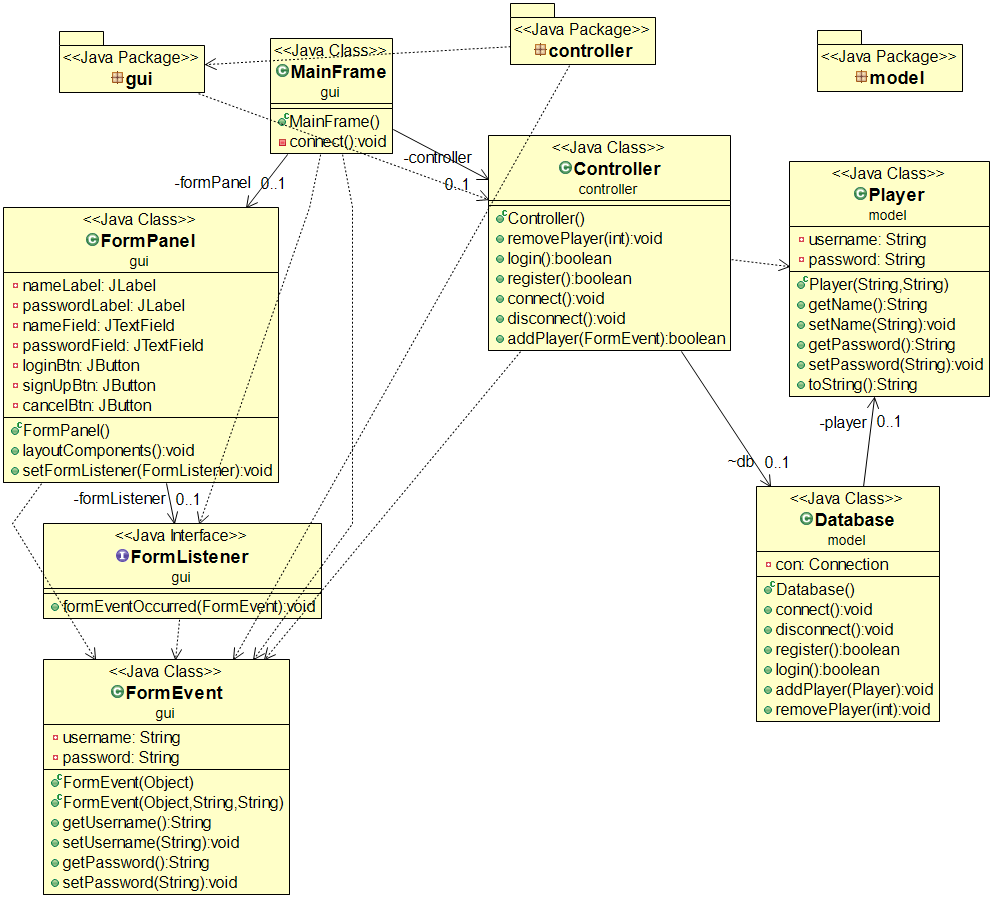
\includegraphics[width=1\textwidth]{images/Registration_UML.png}
    \caption{UML of Registration Subsystems}
    \label{fig:Registration_UML}
\end{figure}

Registration subsystem will be implemented in the iteration 2. This design follows MVC model. The model consists of the Player class and the Database class. The Database class offers the connections to the SQLite database. The gui package is the view of the MVC model, and it is the user interface for the player to login and register. The Controller class controls the data flow between model and view.

\subsubsection{Units Description}

\begin{flushleft}
\begin{tabular}{| l | l | l | l | l |}
    \hline
    \textbf{Class Name} & \multicolumn{4}{ l |} {\textbf{Player}} \\
    \hline
    Inherits from & \multicolumn{4}{ l |}{None} \\
    \hline
    Description & \multicolumn{4}{ l |} {Players can login and register to this game system} \\
    \hline
    \multirow{3}{*}{Attributes} & Visibility & Data Type & Name & Description \\
    \cline{2-5}
     & Private & String & username & Player's username \\
     \cline{2-5}
     & Private & String & password & Player's password \\
    \hline
    \multirow{7}{*}{Methods} & Visibility & Method Name & \multicolumn{2}{l |}{Description} \\
    \cline{2-5}
    & Public & Player(String, String) & \multicolumn{2}{l |}{Constructor} \\
    \cline{2-5}
    & Public & getName() & \multicolumn{2}{l |}{Returns username} \\
    \cline{2-5}
    & Public & setName(String) & \multicolumn{2}{l |}{Sets username} \\
    \cline{2-5}
    & Public & getPassword() & \multicolumn{2}{l |}{Returns password} \\
    \cline{2-5}
    & Public & setPassword(String) & \multicolumn{2}{l |}{Sets password} \\
    \cline{2-5}
    & Public & toString() & \multicolumn{2}{l |}{Returns a string} \\
    \hline
\end{tabular}
\end{flushleft}

\begin{flushleft}
\begin{tabular}{| l | l | l | l | l |}
    \hline
    \textbf{Class Name} & \multicolumn{4}{ l |} {\textbf{Database}} \\
    \hline
    Inherits from & \multicolumn{4}{ l |}{None} \\
    \hline
    Description & \multicolumn{4}{ l |} {A database connection} \\
    \hline
    \multirow{2}{*}{Attributes} & Visibility & Data Type & Name & Description \\
    \cline{2-5}
     & Private & Connection & con &  A connection to database\\
    \hline
    \multirow{8}{*}{Methods} & Visibility & Method Name & \multicolumn{2}{l |}{Description} \\
    \cline{2-5}
    & Public & Database() & \multicolumn{2}{l |}{Constructor} \\
\cline{2-5}
    & Public & connect() & \multicolumn{2}{l |}{Connects to database} \\\cline{2-5}
    & Public & disconnect() & \multicolumn{2}{l |}{Disconnects to database} \\\cline{2-5}
    & Public & register() & \multicolumn{2}{l |}{Registers to game} \\\cline{2-5}
    & Public & login() & \multicolumn{2}{l |}{Login to game} \\\cline{2-5}
    & Public & addPlayer(Player) & \multicolumn{2}{l |}{Inserts a player into database} \\\cline{2-5}
    & Public & removePlayer & \multicolumn{2}{l |}{Deletes a player from database} \\
    \hline
\end{tabular}
\end{flushleft}

\begin{flushleft}
\begin{tabular}{| l | l | l | l | l |}
    \hline
    \textbf{Class Name} & \multicolumn{4}{ l |} {\textbf{Controller}} \\
    \hline
    Inherits from & \multicolumn{4}{ l |}{None} \\
    \hline
    Description & \multicolumn{4}{ l |} {A controller of the Registration subsystem} \\
    % \hline
    % \multirow{2}{*}{Attributes} & Visibility & Data Type & Name & Description \\
    % \cline{2-5}
    %  & Private &  &  &  \\
    \hline
    \multirow{2}{*}{Methods} & Visibility & Method Name & \multicolumn{2}{l |}{Description} \\
    \cline{2-5}
    & Public & Controller() & \multicolumn{2}{l |}{Constructor} \\\cline{2-5}
     & Public & connect() & \multicolumn{2}{l |}{Connects to database} \\\cline{2-5}
    & Public & disconnect() & \multicolumn{2}{l |}{Disconnects to database} \\\cline{2-5}
    & Public & register() & \multicolumn{2}{l |}{Registers to game} \\\cline{2-5}
    & Public & login() & \multicolumn{2}{l |}{Login to game} \\\cline{2-5}
    & Public & addPlayer(FormEvent) & \multicolumn{2}{l |}{Inserts a player into database} \\
    \hline
\end{tabular}
\end{flushleft}

\begin{flushleft}
\begin{tabular}{| l | l | l | l | l |}
    \hline
    \textbf{Class Name} & \multicolumn{4}{ l |} {\textbf{MainFrame}} \\
    \hline
    Inherits from & \multicolumn{4}{ l |}{JFrame} \\
    \hline
    Description & \multicolumn{4}{ l |} {An user interface of the Registration subsystem} \\
    \hline
    % \multirow{2}{*}{Attributes} & Visibility & Data Type & Name & Description \\
    % \cline{2-5}
    %  & Private &  &  &  \\
    % \hline
    \multirow{3}{*}{Methods} & Visibility & Method Name & \multicolumn{2}{l |}{Description} \\
    \cline{2-5}
    & Public & MainFrame() & \multicolumn{2}{l |}{Constructor} \\
    \cline{2-5}
    & Public & connect() & \multicolumn{2}{l |}{Connect to the Controller} \\
    \hline
\end{tabular}
\end{flushleft}

\begin{flushleft}
\begin{tabular}{| l | l | l | l | l |}
    \hline
    \textbf{Class Name} & \multicolumn{4}{ l |} {\textbf{FormPanel}} \\
    \hline
    Inherits from & \multicolumn{4}{ l |}{JPanel} \\
    \hline
    Description & \multicolumn{4}{ l |} {The form panel for players to login and register} \\
    \hline
    \multirow{8}{*}{Attributes} & Visibility & Data Type & Name & Description \\
    \cline{2-5}
     & Private & JLabel & nameLabel & A label \\
     \cline{2-5}
     & Private & JLabel & passwordLabel & A label \\
     \cline{2-5}
     & Private & JTextField & nameField & A text field \\
     \cline{2-5}
     & Private & JTextField & passwordField & A text field \\
     \cline{2-5}
     & Private & JButton & loginBtn & A button \\
     \cline{2-5}
     & Private & JButton & signUpBtn & A button \\
     \cline{2-5}
     & Private & JButton & cancelBtn & A button \\
    \hline
    \multirow{4}{*}{Methods} & Visibility & Method Name & \multicolumn{2}{l |}{Description} \\
    \cline{2-5}
    & Public & FormPanel() & \multicolumn{2}{l |}{Constructor} \\
    \cline{2-5}
    & Public & layoutComponents() & \multicolumn{2}{l |}{Sets the layout components parameters} \\
    \cline{2-5}
    & Public & setFormListener(FormListener) & \multicolumn{2}{l |}{Sets an event listener} \\
    \hline
\end{tabular}
\end{flushleft}

\begin{flushleft}
\begin{tabular}{| l | l | l | l | l |}
    \hline
    \textbf{Class Name} & \multicolumn{4}{ l |} {\textbf{FormEvent}} \\
    \hline
    Inherits from & \multicolumn{4}{ l |}{FormListener} \\
    \hline
    Description & \multicolumn{4}{ l |} {The form events} \\
    \hline
    \multirow{3}{*}{Attributes} & Visibility & Data Type & Name & Description \\
    \cline{2-5}
     & Private & String & username & A username \\
     \cline{2-5}
     & Private & String & password & A password \\
    \hline
    \multirow{7}{*}{Methods} & Visibility & Method Name & \multicolumn{2}{l |}{Description} \\
    \cline{2-5}
    & Public & FormEvent(Object) & \multicolumn{2}{l |}{Constructor} \\
     & Public & FormEvent(Object, String, String) & \multicolumn{2}{l |}{Constructor} \\
    \cline{2-5}
    & Public & getUsername() & \multicolumn{2}{l |}{Returns a username} \\
    \cline{2-5}
    & Public & setUsername() & \multicolumn{2}{l |}{Sets a username} \\
    \cline{2-5}
    & Public & getPassword() & \multicolumn{2}{l |}{Returns a password} \\
    \cline{2-5}
    & Public & setPassword() & \multicolumn{2}{l |}{Sets a password} \\
    \hline
\end{tabular}
\end{flushleft}

\newpage

\subsection{Ranking Subsystem}

\subsubsection{Detailed Design Diagram}


\begin{figure}[htbp]
    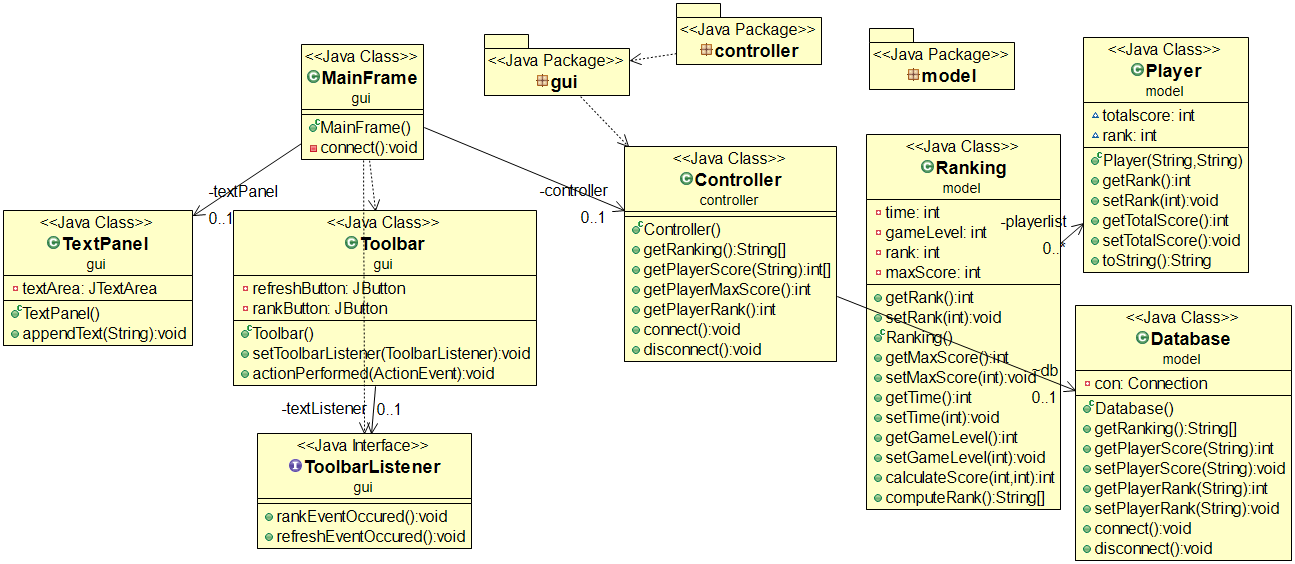
\includegraphics[width=1\textwidth]{images/Ranking_UML.png}
    \caption{UML of Ranking Subsystems}
    \label{fig:Registration_UML}
\end{figure}

The Ranking subsystem design follows the MVC model. The view part consists of the MainFrame, TextPanel, Toolbar and ToolbarListener. The control part is the Controller class and it controls the data flow between the database connection to the MainFrame. The model part consists of the Ranking, Player and Database class. The Ranking class provides the computing ranking functionality. The ranking rules include the time used, the game difficulty level and the correctness of solutions.

\subsubsection{Units Description}

\begin{flushleft}
\begin{tabular}{| l | l | l | l | l |}
    \hline
    \textbf{Class Name} & \multicolumn{4}{ l |} {\textbf{Ranking}} \\
    \hline
    Inherits from & \multicolumn{4}{ l |}{None} \\
    \hline
    Description & \multicolumn{4}{ l |} {To compute the ranking of the players} \\
    \hline
    \multirow{5}{*}{Attributes} & Visibility & Data Type & Name & Description \\
    \cline{2-5}
     & Private & int & time & The time used in a game \\
     \cline{2-5}
     & Private & int & gameLevel & The game difficulty level \\
     \cline{2-5}
     & Private & int & rank & A player's rank position \\
     \cline{2-5}
     & Private & int & maxScore & The maximum score in the system \\
    \hline
    \multirow{12}{*}{Methods} & Visibility & Method Name & \multicolumn{2}{l |}{Description} \\
    \cline{2-5}
    & Public & Ranking() & \multicolumn{2}{l |}{Constructor} \\
    \cline{2-5}
    & Public & getRank() & \multicolumn{2}{l |}{Returns a rank} \\
    \cline{2-5}
    & Public & setRank() & \multicolumn{2}{l |}{Sets a rank} \\
    \cline{2-5}
    & Public & getMaxScore() & \multicolumn{2}{l |}{Returns a highest score} \\
    \cline{2-5}
    & Public & setMaxScore(int) & \multicolumn{2}{l |}{Sets a value} \\
    \cline{2-5}
    & Public & getTime() & \multicolumn{2}{l |}{Returns a time} \\
    \cline{2-5}
    & Public & setTime() & \multicolumn{2}{l |}{Sets a value} \\
    \cline{2-5}
    & Public & getGameLevel() & \multicolumn{2}{l |}{Returns a game difficulty level} \\
    \cline{2-5}
    & Public & setGameLevel(int) & \multicolumn{2}{l |}{Sets a value} \\
    \cline{2-5}
    & Public & calculateScore() & \multicolumn{2}{l |}{Returns a total score} \\
    \cline{2-5}
    & Public & computeRank() & \multicolumn{2}{l |}{Returns a rank according to the rules} \\
    \hline
\end{tabular}
\end{flushleft}

\begin{flushleft}
\begin{tabular}{| l | l | l | l | l |}
    \hline
    \textbf{Class Name} & \multicolumn{4}{ l |} {\textbf{Player}} \\
    \hline
    Inherits from & \multicolumn{4}{ l |}{None} \\
    \hline
    Description & \multicolumn{4}{ l |} {Adds rank and totalscore attributes} \\
    \hline
    \multirow{3}{*}{Attributes} & Visibility & Data Type & Name & Description \\
    \cline{2-5}
     & Private & int & totalscore & The total score of all games for one player \\
     \cline{2-5}
     & Private & int & rank & The rank of a player in the system \\
    \hline
    \multirow{2}{*}{Methods} & Visibility & Method Name & \multicolumn{2}{l |}{Description} \\
    \cline{2-5}
    & Public & getRank() & \multicolumn{2}{l |}{Returns the rank} \\
     \cline{2-5}
    & Public & setRank() & \multicolumn{2}{l |}{Sets a value} \\
    \cline{2-5}
    & Public & getTotalScore() & \multicolumn{2}{l |}{Returns a total score} \\
     \cline{2-5}
    & Public & setTotalScore() & \multicolumn{2}{l |}{Sets a value} \\
     \hline
\end{tabular}
\end{flushleft}

\begin{flushleft}
\begin{tabular}{| l | l | l | l | l |}
    \hline
    \textbf{Class Name} & \multicolumn{4}{ l |} {\textbf{Database}} \\
    \hline
    Inherits from & \multicolumn{4}{ l |}{None} \\
    \hline
    Description & \multicolumn{4}{ l |} {Adds query statements for ranking} \\
    \hline
    \multirow{2}{*}{Attributes} & Visibility & Data Type & Name & Description \\
    \cline{2-5}
     & Private & Connection & con &  A connection to database\\
    \hline
    \multirow{8}{*}{Methods} & Visibility & Method Name & \multicolumn{2}{l |}{Description} \\
    \cline{2-5}
    & Public & Database() & \multicolumn{2}{l |}{Constructor} \\
\cline{2-5}
    & Public & connect() & \multicolumn{2}{l |}{Connects to database} \\\cline{2-5}
    & Public & disconnect() & \multicolumn{2}{l |}{Disconnects to database} \\\cline{2-5}
    & Public & getRanking() & \multicolumn{2}{l |}{Returns a ranking list} \\\cline{2-5}
    & Public & getPlayerScore(String) & \multicolumn{2}{l |}{Returns a score} \\\cline{2-5}
    & Public & setPlayerScore(String) & \multicolumn{2}{l |}{Sets a score in database} \\\cline{2-5}
    & Public & getPlayerRank(String) & \multicolumn{2}{l |}{Returns a rank from database} \\
    \cline{2-5}
    & Public & setPlayerRank(String) & \multicolumn{2}{l |}{Sets a player's rank} \\
    \hline
\end{tabular}
\end{flushleft}

\begin{flushleft}
\begin{tabular}{| l | l | l | l | l |}
    \hline
    \textbf{Class Name} & \multicolumn{4}{ l |} {\textbf{Controller}} \\
    \hline
    Inherits from & \multicolumn{4}{ l |}{None} \\
    \hline
    Description & \multicolumn{4}{ l |} {Adds methods for ranking} \\
    % \hline
    % \multirow{2}{*}{Attributes} & Visibility & Data Type & Name & Description \\
    % \cline{2-5}
    %  & Private &  &  &  \\
    \hline
    \multirow{2}{*}{Methods} & Visibility & Method Name & \multicolumn{2}{l |}{Description} \\
    \cline{2-5}
    & Public & Controller() & \multicolumn{2}{l |}{Constructor} \\\cline{2-5}
     & Public & connect() & \multicolumn{2}{l |}{Connects to database} \\\cline{2-5}
    & Public & disconnect() & \multicolumn{2}{l |}{Disconnects to database} \\\cline{2-5}
    & Public & getRanking() & \multicolumn{2}{l |}{Returns a ranking list} \\\cline{2-5}
    & Public & getPlayerScore(String) & \multicolumn{2}{l |}{Returns a player's total score} \\\cline{2-5}
    & Public & getPlayerMaxScore() & \multicolumn{2}{l |}{Returns a highest score in the system} \\
    \cline{2-5}
    & Public & getPlayerRank(String) & \multicolumn{2}{l |}{Return a player's rank} \\
    \hline
\end{tabular}
\end{flushleft}

\begin{flushleft}
\begin{tabular}{| l | l | l | l | l |}
    \hline
    \textbf{Class Name} & \multicolumn{4}{ l |} {\textbf{MainFrame}} \\
    \hline
    Inherits from & \multicolumn{4}{ l |}{JFrame} \\
    \hline
    Description & \multicolumn{4}{ l |} {An user interface of the Registration subsystem} \\
    \hline
    % \multirow{2}{*}{Attributes} & Visibility & Data Type & Name & Description \\
    % \cline{2-5}
    %  & Private &  &  &  \\
    % \hline
    \multirow{3}{*}{Methods} & Visibility & Method Name & \multicolumn{2}{l |}{Description} \\
    \cline{2-5}
    & Public & MainFrame() & \multicolumn{2}{l |}{Constructor} \\
    \cline{2-5}
    & Public & connect() & \multicolumn{2}{l |}{Connect to the Controller} \\
    \hline
\end{tabular}
\end{flushleft}

\begin{flushleft}
\begin{tabular}{| l | l | l | l | l |}
    \hline
    \textbf{Class Name} & \multicolumn{4}{ l |} {\textbf{TextPanel}} \\
    \hline
    Inherits from & \multicolumn{4}{ l |}{JPanel} \\
    \hline
    Description & \multicolumn{4}{ l |} {Displays a ranking list in the text area} \\
    \hline
    \multirow{2}{*}{Attributes} & Visibility & Data Type & Name & Description \\
    \cline{2-5}
     & Private & JTextArea & textArea & A text area \\
    \hline
    \multirow{3}{*}{Methods} & Visibility & Method Name & \multicolumn{2}{l |}{Description} \\
    \cline{2-5}
    & Public & TextPanel() & \multicolumn{2}{l |}{Constructor} \\
    \cline{2-5}
    & Public & appendText(String) & \multicolumn{2}{l |}{Appends text} \\
    \hline
\end{tabular}
\end{flushleft}

\begin{flushleft}
\begin{tabular}{| l | l | l | l | l |}
    \hline
    \textbf{Class Name} & \multicolumn{4}{ l |} {\textbf{Toolbar}} \\
    \hline
    Inherits from & \multicolumn{4}{ l |}{JPanel} \\
    \hline
    Description & \multicolumn{4}{ l |} {A toolbar with buttons} \\
    \hline
    \multirow{3}{*}{Attributes} & Visibility & Data Type & Name & Description \\
    \cline{2-5}
     & Private & JButton & refreshButton & A refresh button \\
     \cline{2-5}
     & Private & JButton & rankButton & A rank button \\
    \hline
    \multirow{2}{*}{Methods} & Visibility & Method Name & \multicolumn{2}{l |}{Description} \\
    \cline{2-5}
    & Public & Toolbar() & \multicolumn{2}{l |}{Constructor} \\
    \cline{2-5}
    & Public & setToolbarListener(ToolbarListener) & \multicolumn{2}{l |}{Sets event listener} \\
    \cline{2-5}
    & Public & actionPerformed(ActionEvent) & \multicolumn{2}{l |}{Performs actions} \\
    \hline
\end{tabular}
\end{flushleft}

\begin{flushleft}
\begin{tabular}{| l | l | l | l | l |}
    \hline
    \textbf{Interface Name} & \multicolumn{4}{ l |} {\textbf{ToolbarListener}} \\
    \hline
    Inherits from & \multicolumn{4}{ l |}{None} \\
    \hline
    Description & \multicolumn{4}{ l |} {} \\
    \hline
    % \multirow{2}{*}{Attributes} & Visibility & Data Type & Name & Description \\
    % \cline{2-5}
    %  & Private &  &  &  \\
    % \hline
    \multirow{3}{*}{Methods} & Visibility & Method Name & \multicolumn{2}{l |}{Description} \\
    \cline{2-5}
    & Public & rankEventOccured() & \multicolumn{2}{l |}{Listens the rank button} \\
    \cline{2-5}
    & Public & refreshEventOccured() & \multicolumn{2}{l |}{Listens the refresh button} \\
    \hline
\end{tabular}
\end{flushleft}

\newpage

\section{Dynamic Design Scenarios}
The following are the descriptions of the execution scenarios of the game initialization, the process of saving a game and the process of loading a game. These systems are involved in the subsystem of the puzzle mechanics.

**FIX initialize game
**add: play GAME ***
**Do introduction



\subsection{Initialize Game (UI only)}
\begin{figure}[htbp]
    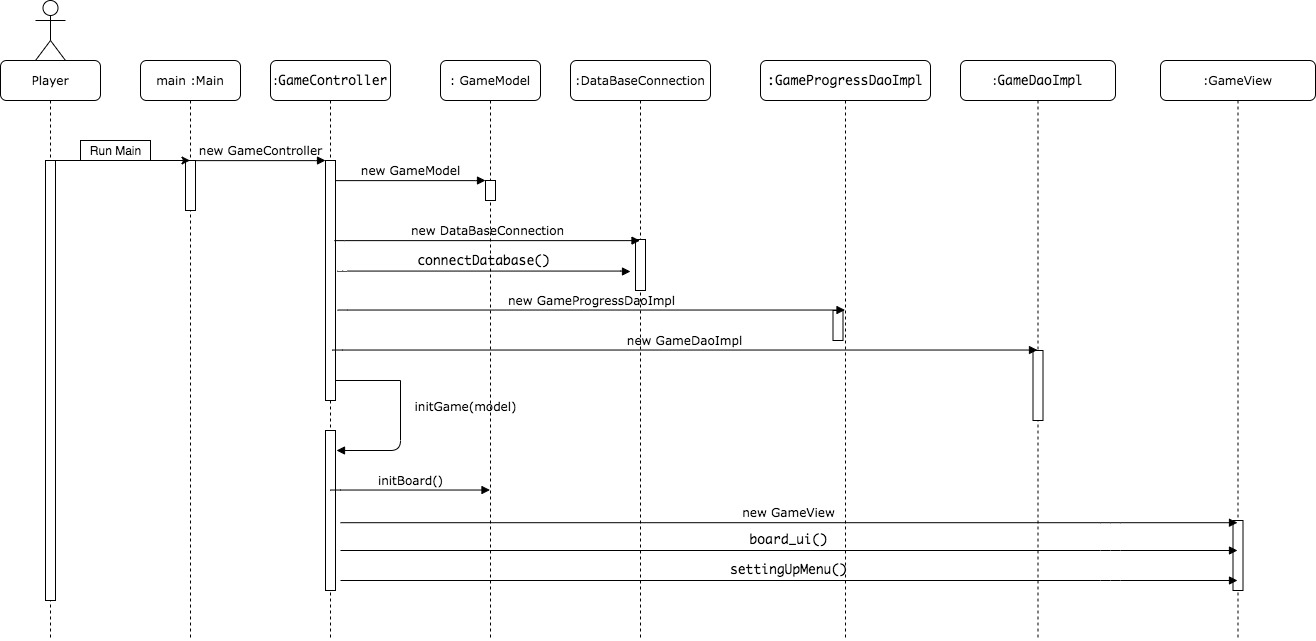
\includegraphics[width=1\textwidth]{initializeGame_UI}
    \caption{Sequence diagram to initialize a game}
    \label{fig:sequenceDiagram}
\end{figure}

\newpage

\subsection{Save Game}
\begin{figure}[htbp]
    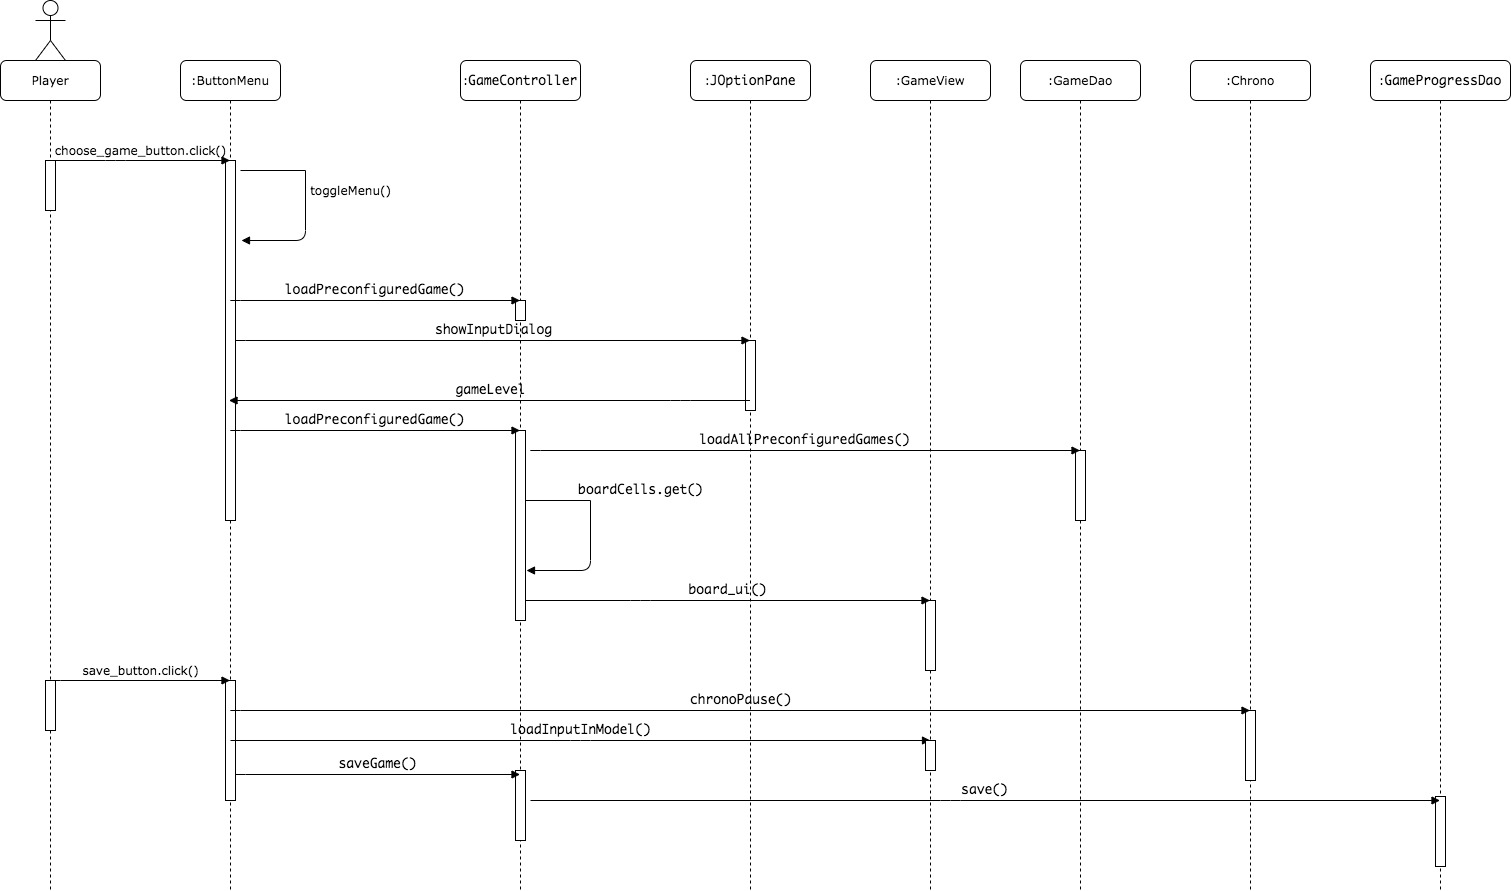
\includegraphics[width=1\textwidth]{saveGame}
    \caption{Sequence diagram to save a game}
    \label{fig:sequenceDiagram}
\end{figure}

\newpage

\subsection{Load Game}
\begin{figure}[htbp]
    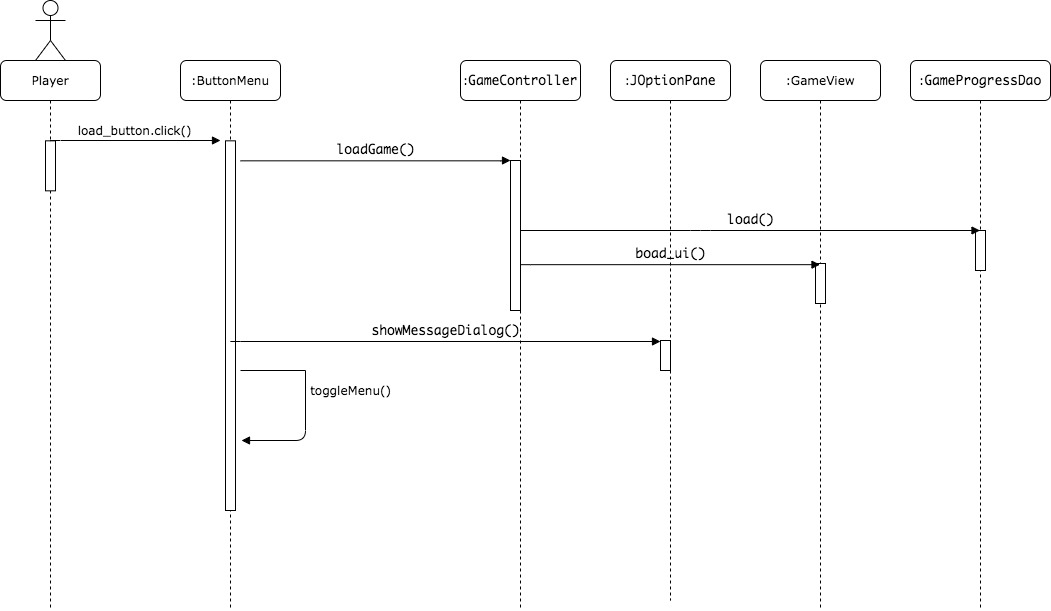
\includegraphics[width=1\textwidth]{loadGame}
    \caption{Sequence diagram to load a game}
    \label{fig:sequenceDiagram}
\end{figure}
\end{document}
